\insertmeeting 
	{Meeting Example} 
	{02/01/23} 
	{Hagerty High School}
	{JenseLauran}
	{Images/RobotPics/robot.jpg}
	{2:30 - 4:30}
	
\hhscommittee{Hardware}
\noindent\hfil\rule{\textwidth}{.4pt}\hfil
\subsubsection*{Goals}
\begin{itemize}
    \item Finish CAD of drive plane plates
    \item Continue working on vision
\end{itemize} 

\noindent\hfil\rule{\textwidth}{.4pt}\hfil

\subsubsection*{Accomplishments}
Today, the team began working on the new lift after Leagues. We CADed the rollers and the panels for the poles, and began to work on the servo plate in the center. Work on the lift is being stalled until the poles are placed onto the drive train, which was first designed in CAD. The drive train plate will soon be finished up. Software has began their fine tuning of the autonomous, where they revised vision, and programmed the picking up and placement of the cones.
 

\begin{figure}[ht]
\centering
\begin{minipage}[b]{.48\textwidth}
  \centering
  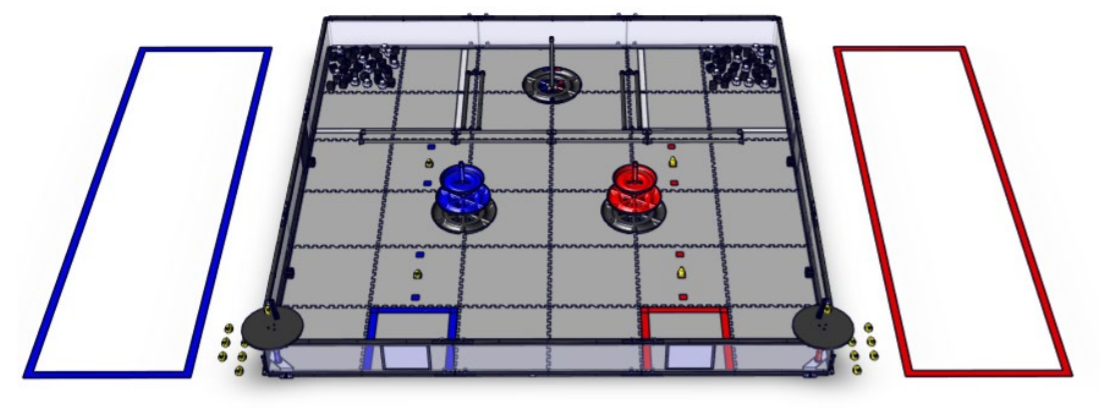
\includegraphics[width=0.95\textwidth]{Meetings/January/01-01-22/field.png}
  \caption{New Account in Github}
  \label{fig:pic1}
\end{minipage}%
\hfill%
\begin{minipage}[b]{.48\textwidth}
  \centering
  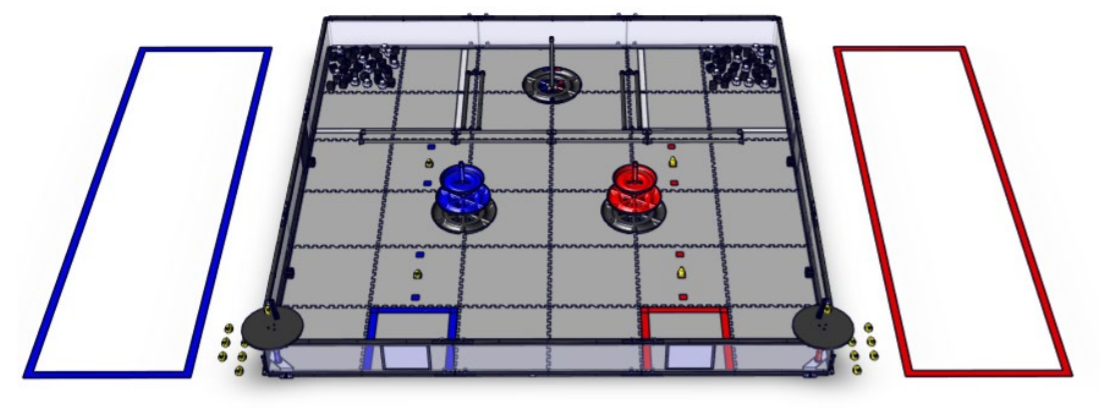
\includegraphics[width=0.95\textwidth]{Meetings/January/01-01-22/field.png}
  \caption{Screenshot of GitHub Repository}
  \label{fig:pic2}
\end{minipage}
\end{figure}

\whatsnext{
\begin{itemize}
    \item Laser cut intake parts
    \item 3d print intake parts
    \item Build intake
\end{itemize} 
}

